% Made up for the tikra benchmark.
\usetikzlibrary{patterns}
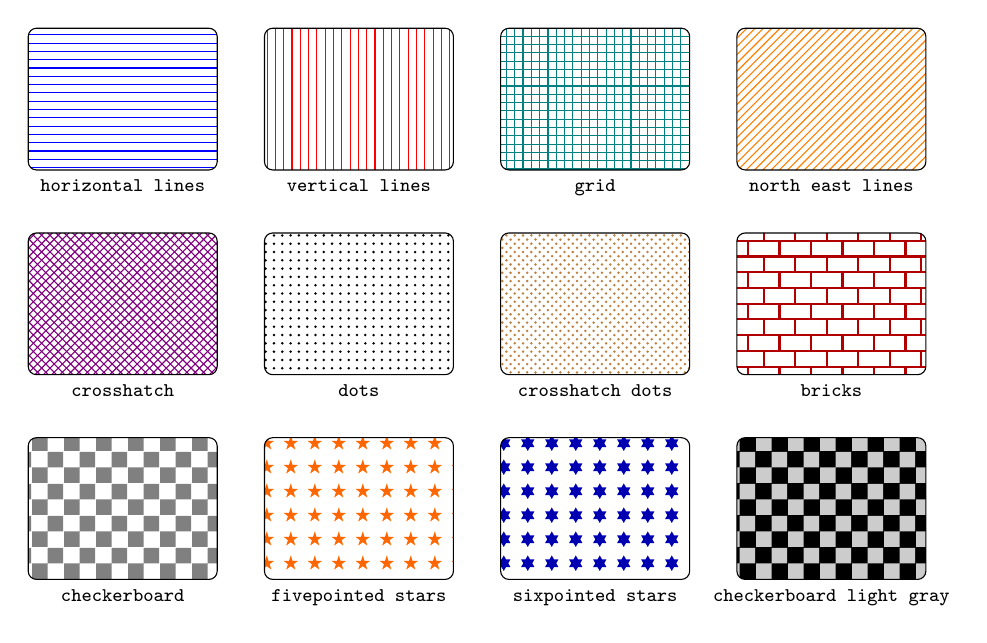
\begin{tikzpicture}
  \foreach \p/\c [count=\i from 0] in {horizontal lines/blue, vertical lines/red, grid/teal,
      north east lines/orange, crosshatch/violet, dots/black, crosshatch dots/brown,
      bricks/red!70!black, checkerboard/gray, fivepointed stars/orange!80!red,
      sixpointed stars/blue!70!black, checkerboard light gray/black} {
    \pgfmathsetmacro\x{mod(\i,4)*3}
    \pgfmathsetmacro\y{-int(\i/4)*2.6}
    \draw[pattern=\p, pattern color=\c, rounded corners=3pt] (\x,\y) rectangle +(2.4,1.8);
    \node[font=\scriptsize\ttfamily, below] at (\x+1.2,\y) {\p};
  }
\end{tikzpicture}
